\documentclass[a4paper,12pt]{article}
%\usepackage[latin1]{inputenc}
\usepackage[spanish]{babel}
\usepackage{bm}
\usepackage{graphicx}
\usepackage{amsmath}
\spanishdecimal{.}
\setlength{\textheight}{235mm}
\setlength{\textwidth}{168mm}
\setlength{\oddsidemargin}{0pt}
\pagestyle{empty}
\begin{document}
\mbox{}\vspace*{-45mm}

{\centering
{\small\sc Escuela Técnica Superior de Ingenieros de Caminos, Canales y
Puertos (Madrid)}\\*[4mm]
{\Large\bf Método de los Elementos Finitos (Curso 23-24)}\\*[4mm]
Ejercicio 2: Ecuación de difusión \\*[4mm]
}

\vspace{3mm}

%%%%%
\noindent

Se dispone una presa sobre un terreno tal que aguas arriba se almacena el agua a una cierta altura. Aguas abajo de la presa el nivel de agua coincide con el terreno natural. Se instaló una pantalla impermeable (profundidad igual a 5m y espesor igual a 0.05m) debajo de la presa en la zona de aguas abajo, como muestra la figura. Las unidades de la figura son en metros.   
El terreno está formado por dos materiales distintos; un estrato menos permeable debajo de la base de la presa ($K_1$ = $1\cdot 10^{-4}$ m/s) y otro donde se instaló la pantalla ($K_2$ = $1\cdot 10^{-3}$ m/s).

Se asumirá que los contornos laterales del terreno, así como la base del mismo, son impermeables.


\vspace{0.4cm}

\begin{center}
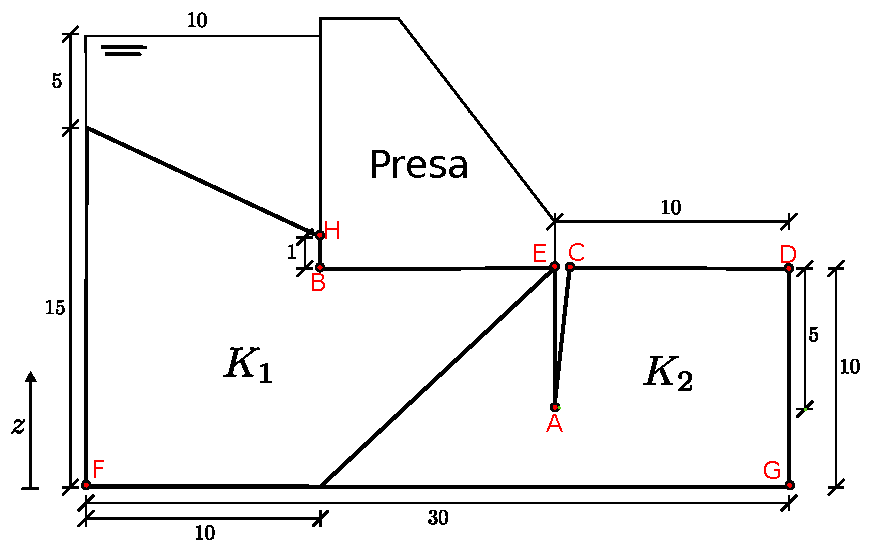
\includegraphics[width=1\textwidth]{Ejer2._2023-cropped.pdf}
\end{center}
\vspace{0.4cm}

Téngase en cuenta las siguientes consideraciones:

\begin{itemize}
\item Se usarán elementos cuadriláteros con tamaño global de malla de 1 metro e
  interpolación lineal. 
\item Se considerará que el fluido es agua dulce con densidad $\rho_w=1000$
  kg/m$^3$ y que el valor de la aceleración de la gravedad vale $g=9.81$ m/s$^2$.

\end{itemize}

\end{document}